\documentclass{article}

\usepackage[utf8x]{inputenc}
\usepackage[T1]{fontenc}
\usepackage[francais]{babel}
\usepackage{xcolor}
\usepackage{listings}
\usepackage{mathptmx}
\usepackage{anyfontsize}
\usepackage{t1enc}
\usepackage[top=2cm, bottom=2cm, left=2cm, right=2cm]{geometry}
\usepackage{titlesec}
\usepackage{titling}
\usepackage{graphicx}
\usepackage{pgfplots}
\usepackage[colorlinks = true,
            linkcolor = black,
            urlcolor  = black,
            citecolor = black,
            anchorcolor = black]{hyperref}

\newcommand{\changeurlcolor}[1]{\hypersetup{urlcolor=#1}}

\renewcommand\maketitlehooka{\null\mbox{}\vfill}
\renewcommand\maketitlehookd{\vfill\null}

\definecolor{codegreen}{rgb}{0,0.6,0}
\definecolor{codegray}{rgb}{0.5,0.5,0.5}
\definecolor{codepurple}{rgb}{0.58,0,0.82}
\definecolor{backcolour}{rgb}{0.95,0.95,0.92}
\definecolor{codekeywords}{rgb}{0.1,0.53,0.92}

\lstdefinestyle{c++}{
    backgroundcolor=\color{backcolour},   
    commentstyle=\color{codegreen},
    keywordstyle=\color{codekeywords},
    numberstyle=\tiny\color{codegray},
    stringstyle=\color{codepurple},
    basicstyle=\ttfamily\footnotesize,
    breakatwhitespace=false,         
    breaklines=true,                 
    captionpos=b,                    
    keepspaces=true,                 
    numbers=left,                    
    numbersep=5pt,                  
    showspaces=false,                
    showstringspaces=false,
    showtabs=false,                  
    tabsize=2,
    texcl=false,
    inputencoding=utf8,
    extendedchars=true,
    literate=
  {á}{{\'a}}1 {é}{{\'e}}1 {í}{{\'i}}1 {ó}{{\'o}}1 {ú}{{\'u}}1
  {Á}{{\'A}}1 {É}{{\'E}}1 {Í}{{\'I}}1 {Ó}{{\'O}}1 {Ú}{{\'U}}1
  {à}{{\`a}}1 {è}{{\`e}}1 {ì}{{\`i}}1 {ò}{{\`o}}1 {ù}{{\`u}}1
  {À}{{\`A}}1 {È}{{\'E}}1 {Ì}{{\`I}}1 {Ò}{{\`O}}1 {Ù}{{\`U}}1
  {ä}{{\"a}}1 {ë}{{\"e}}1 {ï}{{\"i}}1 {ö}{{\"o}}1 {ü}{{\"u}}1
  {Ä}{{\"A}}1 {Ë}{{\"E}}1 {Ï}{{\"I}}1 {Ö}{{\"O}}1 {Ü}{{\"U}}1
  {â}{{\^a}}1 {ê}{{\^e}}1 {î}{{\^i}}1 {ô}{{\^o}}1 {û}{{\^u}}1
  {Â}{{\^A}}1 {Ê}{{\^E}}1 {Î}{{\^I}}1 {Ô}{{\^O}}1 {Û}{{\^U}}1
  {œ}{{\oe}}1 {Œ}{{\OE}}1 {æ}{{\ae}}1 {Æ}{{\AE}}1 {ß}{{\ss}}1
  {ç}{{\c c}}1 {Ç}{{\c C}}1 {ø}{{\o}}1 {å}{{\r a}}1 {Å}{{\r A}}1
  {€}{{\EUR}}1 {£}{{\pounds}}1,
}
\lstset{style=c++}


\title{Simulation TP4\\Simulation d'une population de lapins}
\author{Arquillière Mathieu}
\date{\today}

\begin{document}

\begin{titlepage}
  \maketitle
\end{titlepage}

\tableofcontents
\newpage
\listoffigures
\newpage

\section{Introduction}
L'objectif de ce TP est de modéliser à l'aide de la programmation objet
des lapins afin d'étudier le comportement d'une population. Pour la gestion
de l'aléatoire, on utilisera la bibliothèque \emph{random} fournie par la
STL du c++. On utilisera le générateur \emph{std::mt19937} Mersenne Twister
et les distributions uniformes et normales.

\section{Analyse du sujet}
Il s'agit de simuler le comportement d'une population de lapins sans prédateurs.
Il y a plusieurs parties à comprendre et à implémenter.

\subsection{Naissances}
Le sujet nous indique qu'une femelle lapin peut donner 4 à 8 portées par an, avec
une probabilité plus forte de faire 4, 5 ou 6 portées. De plus, chaque portée
peut donner 3 à 6 bébés lapins avec une 50\% de chance d'être un mâle et 50\%
de chance d'être une femelle pour chaque bébé lapin.

\subsection{Majorité}
Un lapin devient adulte au bout d'un certain nombre de mois, compris
aléatoirement entre 5 et 8 mois. Cette majorité sert à la fois pour les
naissances puisqu'une femelle ne peut enfanter qu'à partir de se majorité
si il y a au moins 1 lapin mâle également adulte, mais aussi pour la
probabilité de mourir.

\subsection{Mort}
Un lapin a 20\% de chance de mourir lors de sa jeunesse (donc sur les 5
à 8 mois avant la majorité). Lorsqu'il atteint l'âge adulte, il a 50\% de
chance de mourir. On considérera que ce chiffre correspond à l'âge adulte
en entier, c'est à dire 11 ans moins le nombre de mois de jeunesse. A partir
de 11 ans il rentre dans l'âge "vieux" et cette probabilité de mourir
augmente de 10\% chaque année (fatalement, il meurt donc forcément à 15 ans).

\section{Implémentation}
De façon générale, on exécutera les tests en nombre de mois.

\subsection{L'objet lapin}
L'objet lapin représentera un lapin, quelque soit son genre. Il contient
donc un attribut \emph{age} et un attribut \emph{majorité} en nombre de mois.
Il contient également les probabilités de mourir jeune et en étant adulte
puisque celles-ci sont calculées en fonction de la majorité. Pour ce qui
est des méthodes, la classe a besoin de \emph{grow()} qui sera appelée tous les
mois pour faire grandir le lapin, elle a besoin d'une méthode permettant
de savoir si le lapin doit mourir ce mois (\emph{hasToDie()}) et enfin
de 2 méthodes utilitaire, l'une pour savoir si le lapin est adulte
(\emph{hasMajority()}) et l'autre pour obtenir l'age (\emph{getAge()}) qui
sera surtout utilisée pour faire des statistiques. La classe contient aussi
les probabilités de survie afin de faciliter le changement de paramètres
pour exécuter des simulations différentes et éviter les \emph{magic numbers}.

A la base, cette classe est destinée à être la classe mère réunissant les
classes filles \emph{lapin femelle} et \emph{lapin mâle}. Cependant même si
effectivement la classe du lapin femelle ajoute beaucoup de "fonctionnalités",
le mâle n'a pas besoin d'une classe spécifique. Ainsi, une instance de la
classe \emph{Rabbit} correspond à un lapin mâle, et il faut créer une classe
\emph{FemaleRabbit} héritant de la classe \emph{Rabbit} qui elle correspond
à un lapin femelle.

\begin{figure}[!h]
  \centering
  \caption{Déclaration de la classe \emph{Rabbit}}
  \lstinputlisting[language=c++, firstline=16, lastline=43]{Rabbit.hpp}
\end{figure}

\newpage

La plupart des implémentations des méthodes de cette classe sont assez simples
(\emph{getAge()} renvoie l'age, \emph{grow()} augmente l'age de 1). Le constructeur
lui est un peu plus spécial. En effet c'est dans celui-ci qu'on décide de
la majorité et donc les probilités de mort. Puisque notre unité de temps
est le mois, on redéfinit les probabilités du sujet pour obtenir une probabilité
par mois.
$$
(P_{jeune})^{majorite} = 0.2 \Leftrightarrow P_{jeune} = 0.2^{majorite}
$$
$$
(P_{adulte})^{11 ans - majorite} = 0.5 \Leftrightarrow P_{adulte} = 0.2^{132 - majorite}
$$

\begin{figure}[!h]
  \caption{Constructeur de la classe \emph{Rabbit}}
  \lstinputlisting[language=c++, firstline=13, lastline=24]{Rabbit.cpp}
\end{figure}

\newpage
\subsection{L'objet Lapin femelle}
L'objet \emph{FemaleRabbit} est une spécification de la classe \emph{Rabbit}. En effet, elle
rajoute la possibilité de donner naissance. Pour ça, elle a besoin d'une référence sur la
liste contenant la population (pour y rajouter ses enfants) qu'on lui passe en paramètre
lorsqu'on créer une instance.

\begin{figure}[!h]
  \caption{Déclaration de la classe \emph{FemaleRabbit}}
  \lstinputlisting[language=c++, firstline=17, lastline=34]{FemaleRabbit.hpp}
\end{figure}

Elle redéfinit également la méthode \emph{grow()}. Celle-ci permet ainsi de grandir
(en appelant la méthode de \emph{Rabbit}) mais aussi d'enfanter. Afin de simplifier le
fait de donner des portées 4 à 8 fois par an avec plus de probabilités pour 5, 6 ou 7 mois,
on décide 1 fois par an le nombre de portées que la femelle aura dans l'année avec une
distribution normale.

\begin{figure}[!h]
  \centering
  \caption{Exemple d'utilisation de distribution normale en C++ (voir \href{https://en.cppreference.com/w/cpp/numeric/random/normal\_distribution}{cppreference})}
  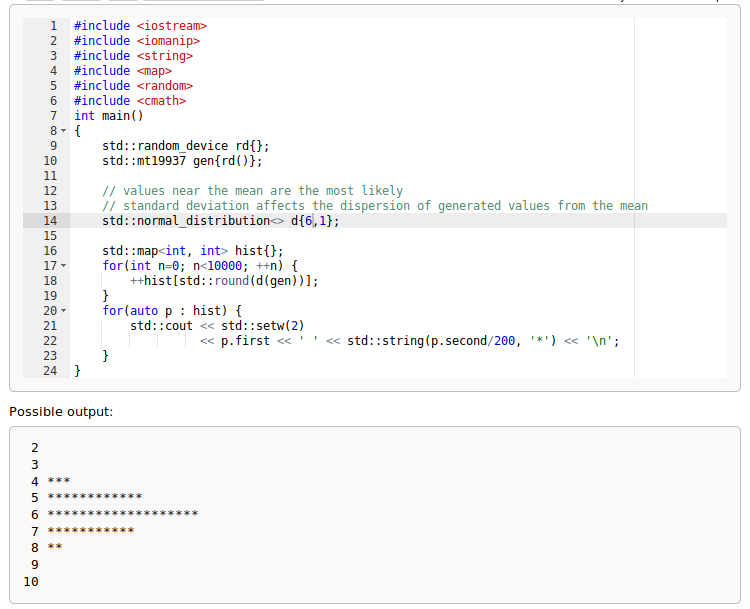
\includegraphics[scale=0.5]{normal_dist.png}
\end{figure}

\newpage
Une fois le nombre de portées décidé, on décide aléatoirement avec une distribution uniforme
entre 0 et 11 les mois auquels la femelle donne une portée. On stocke ces informations avec
un tableau de booléens correspondant au mois. Ainsi chaque mois (donc dans cette même fonction
\emph{grow()}), on teste si la femelle doit enfanter (\emph{true} dans le tableau) et dans ce
cas, on décide aléatoirement suivant une loi uniforme entre 3 et 6 le nombre de bébés de la portée.

\begin{figure}[!h]
  \caption{Méthode \emph{grow()} de \emph{FemaleRabbit}}
  \lstinputlisting[language=c++, firstline=35, lastline=79]{FemaleRabbit.cpp}
\end{figure}

\subsection{L'objet Population}
Maintenant, afin de gérer un ensemble de lapins et de les faire interargir, on créé
un objet \emph{Population}. On utilisera une liste (\emph{std::list}) de la STL afin
de stocker des pointeurs sur des lapins. Une liste a l'avantage d'avoir l'insertion /
suppression en \emph{O(1)}. Cette classe démarrera avec 1 lapin mâle et 1 lapin femelle ou avec
un nombre de lapins de chaque sexe donné. Ensuite elle se chargera de "faire passer le temps"
aux lapins et de récuperer un certain nombre d'informations comme le nombre de morts ou de
naissances.

\begin{figure}[!h]
  \caption{Déclaration de la classe \emph{Population}}
  \lstinputlisting[language=c++, firstline=19, lastline=50]{Population.hpp}
\end{figure}


Afin de "faire passer le temps" aux lapins, on appelle la méthode \emph{grow()} chaque mois
pour chaque lapin, méthode qui peut ajouter des lapins dans la liste grâce aux femelles, et
d'appeler la méthode \emph{hasToDie()} pour tester si le mois passé fais mourir des lapins.
Ces lapins sont détruits et retirés de la liste.

\begin{figure}[!h]
  \caption{Implémentation de la méthode \emph{passTime}, boucle principale faisant grandir la population}
  \lstinputlisting[language=c++, firstline=59, lastline=98]{Population.cpp}
\end{figure}

\newpage
\section{Résultats}
\subsection{Tests simple d'une population}
Si on observe l'évolution d'une population simple, prenons par exemple 2000 lapins au départ avec
1000 mâles et 1000 femelles, sur 100 mois, alors on observe qu'à partir d'un certain mois
(aux environs de 40-50), la courbe démographique ressemble à une exponentielle.

\begin{center}
  \centering
  \begin{figure}[h]
  \caption{Evolution de population avec 1000 mâles / 1000 femelles au départ et sur 100 mois}
\begin{tikzpicture}
  \begin{axis}[
    enlarge x limits=false,
    width=1\textwidth,
    height=0.4\textwidth,
    xlabel={Mois},
    ylabel={Nombre de lapins},
    ymax=1500000
  ]
  \addplot file{100months_1000-1000.txt};
  \end{axis}
\end{tikzpicture}
\end{figure}
\end{center}

\newpage
Si on zoom un peu sur les 50 premiers mois, on obtient un graphique qui nous permet de voir
que la population décroit un peu au début puis part en exponentielle. On peut sans doute
expliquer cela du fait que les femelles ne peuvent pas enfanter tout de suite, puisqu'elles
doivent atteindre la majorité. Ainsi dès que les premiers enfants arrivent dans la population,
il y a plus de naissances que de morts, donc la population augmente  de façon exponentielle.

\begin{center}
\begin{figure}[!h]
\caption{Evolution de population avec 1000 mâles / 1000 femelles au départ et sur 50 mois}
\begin{tikzpicture}
  \begin{axis}[
    enlarge x limits=false,
    width=1\textwidth,
    height=0.6\textwidth,
    xlabel={Mois},
    ylabel={Nombre de lapins},
    ymax=20000,
    bar width=8pt
  ]
  \addplot[ybar] file{50months_1000-1000.txt};
  \end{axis}
\end{tikzpicture}
\end{figure}
\end{center}

\subsection{Tests sur plusieurs populations}
On peut également observer le nombre moyens de lapins dans une population au bout d'un certain
nombre de mois. Le principe est simple, on a une boucle où l'on créé une population à chaque itération
, on lui fait passer un certain nombre de mois et on garde les statistiques à la fin. Par exemple,
on peut observer les moyennes pour 20 populations à 50 mois:
\begin{lstlisting}[language=c++]
20 populations sur 50 mois:
Moyenne du nombre de lapins:            23241.8
Moyenne du nombre de mâles:             11607.5
Moyenne du nombre de femelles:          11634.4
Moyenne du nombre de morts:             45436.2
Moyenne du nombre de naissances:        68678
Moyenne des moyennes d age de mort:     2.6958
\end{lstlisting}
On observe que la répartition mâle / femelles est en effet de 50/50. On voit aussi qu'il y a
plus de mort que de naissance. Voici un autre exemple avec 10 itérations de 100 mois:
\begin{lstlisting}[language=c++]
10 populations sur 100 mois:
Moyenne du nombre de lapins:            1.496e+06
Moyenne du nombre de mâles:             747749
Moyenne du nombre de femelles:          748252
Moyenne du nombre de morts:             2.91845e+06
Moyenne du nombre de naissances:        4.41445e+06
Moyenne des moyennes d age de mort:     2.70848
\end{lstlisting}

\section{Conclusion}
Malheureusement, pour faire une serie de tests plus concluants, il faudrait regarder beaucoup
plus de paramètre et exécuter des tests plus variés (le nombre de lapins au départ, le nombre
de mois, les probabilités de mourir, ...). De plus les simulations sont assez limitées par le
temps d'exécution du programme. En effet au delà de 120 mois, il y a trop de lapins à mettre à jour
et l'implémentation prends trop de temps. Il est par contre possible de réflechir à d'autres
implémentations. Par exemple, il sera possible de "pré-générer" les lapins lors de leurs naissance
en choisissant toute sa vie à l'avance (ses dates d'accouchements, sa date de mort, ...) et ainsi
éviter beaucoup de tests inutiles.

Il serait également intéressant de transformer l'implémentation actuelle avec des \emph{templates}
afin de choisir des conteneurs de populations différents (\emph{list, forward-list, vector, deque})
et d'évaluer lesquelles sont les plus efficaces.



\newpage
\appendix
\section{Manuel d'utilisation}
Le programme possède 2 sortes d'utilisation, une avec 1 population et une autre en en faisant plusieurs.

\subsection{Gestion d'une seule population}
Si on veut regarder l'évolution d'une population sur 50 mois
\begin{lstlisting}[language=c++]
  ./lapin.exe
\end{lstlisting}
Si on veut préciser le nom du fichier de sortie
\begin{lstlisting}[language=c++]
  ./lapin.exe fichierSortie.txt
\end{lstlisting}
Si on veut préciser le nombre de mois à passer (il faut obligatoirement un nom de fichier si on veut indiquer ce nombre)
\begin{lstlisting}[language=c++]
  ./lapin.exe fichierSortie.txt 100
\end{lstlisting}

\subsection{Moyenne sur plusieurs populations}
Si on veut observer les statistiques de plusieurs évolutions de populations (par défaut 10 populations sur 50 mois)
\begin{lstlisting}[language=c++]
  ./lapin.exe -s
\end{lstlisting}
Si on préciser le nombre de populations qu'on veut observer
\begin{lstlisting}[language=c++]
  ./lapin.exe -s 20
\end{lstlisting}
Si on préciser le nombre de mois qu'on passe pour chaque population (il faut obligatoirement mettre le nombre de populations aussi)
\begin{lstlisting}[language=c++]
  ./lapin.exe -s 20 100
\end{lstlisting}

\section{Compilation}
Un makefile a été utilisé pour simplifier la compilation de ce TP. Voici son contenu
\lstinputlisting[language=c++]{makefile}

On a seulement besoin de la STL du c++. Notamment de la bibliothèque \href{https://en.cppreference.com/w/cpp/numeric/random}{\emph{<random>}}
pour générer tous les nombre pseudo-aléatoires du programme, de la bibliothèque \href{https://en.cppreference.com/w/cpp/container/list}{\emph{<list>}}
et de \href{https://en.cppreference.com/w/cpp/algorithm}{\emph{<algorithm>}} afin de gérer les populations.

\section{Documentation}
\changeurlcolor{blue}\href{run:Documentation.pdf}{Lien vers la documentation Doxygen}

\end{document}
